\documentclass[11pt]{beamer}
\usepackage{float}
\usepackage{graphicx}
\usepackage{dcolumn}
\usepackage{array}  
\newcolumntype{.}{D{.}{.}{-1}}

\setbeamertemplate{footline}[frame number]

\AtBeginSection[]
{
  \begin{frame}
    \frametitle{Table of Contents}
    \tableofcontents[currentsection]
  \end{frame}
}

\title{Assignment Beamer Presentation}
\author{Yusi Qin, Xiwei Wang, Jin Zhang}
\institute{University of Zurich}
\date{\today}

\begin{document}

\frame{\titlepage}

\begin{frame}
\frametitle{Table of Contents}
\tableofcontents
\end{frame}

\section{Figures}

\subsection{Tips}
\begin{frame}
\frametitle{Tips}
\begin{itemize}
    \item Use 11pt fonts in beamer.
    \item Never text in the bottom right corner. The most important part in a page should be the top left corner and the center. 
    \item Beware of the colorblindness.
    \item Form a pattern, try to be stable. e.g. Tesla is consistent with blue in all figures. 
    \item Tables should be consistent.
    \item associate good values to warm colors while bad to cold colors.
    \item specific cultures: associate Coca Cola to red.
\end{itemize}
\end{frame}

\subsection{Colorblindness}
\begin{frame}{Colorblindness}
After implementing seaborn colorblindness palette.(corresponding code in ipynb file)
\begin{figure}[htbp]
        \centering
        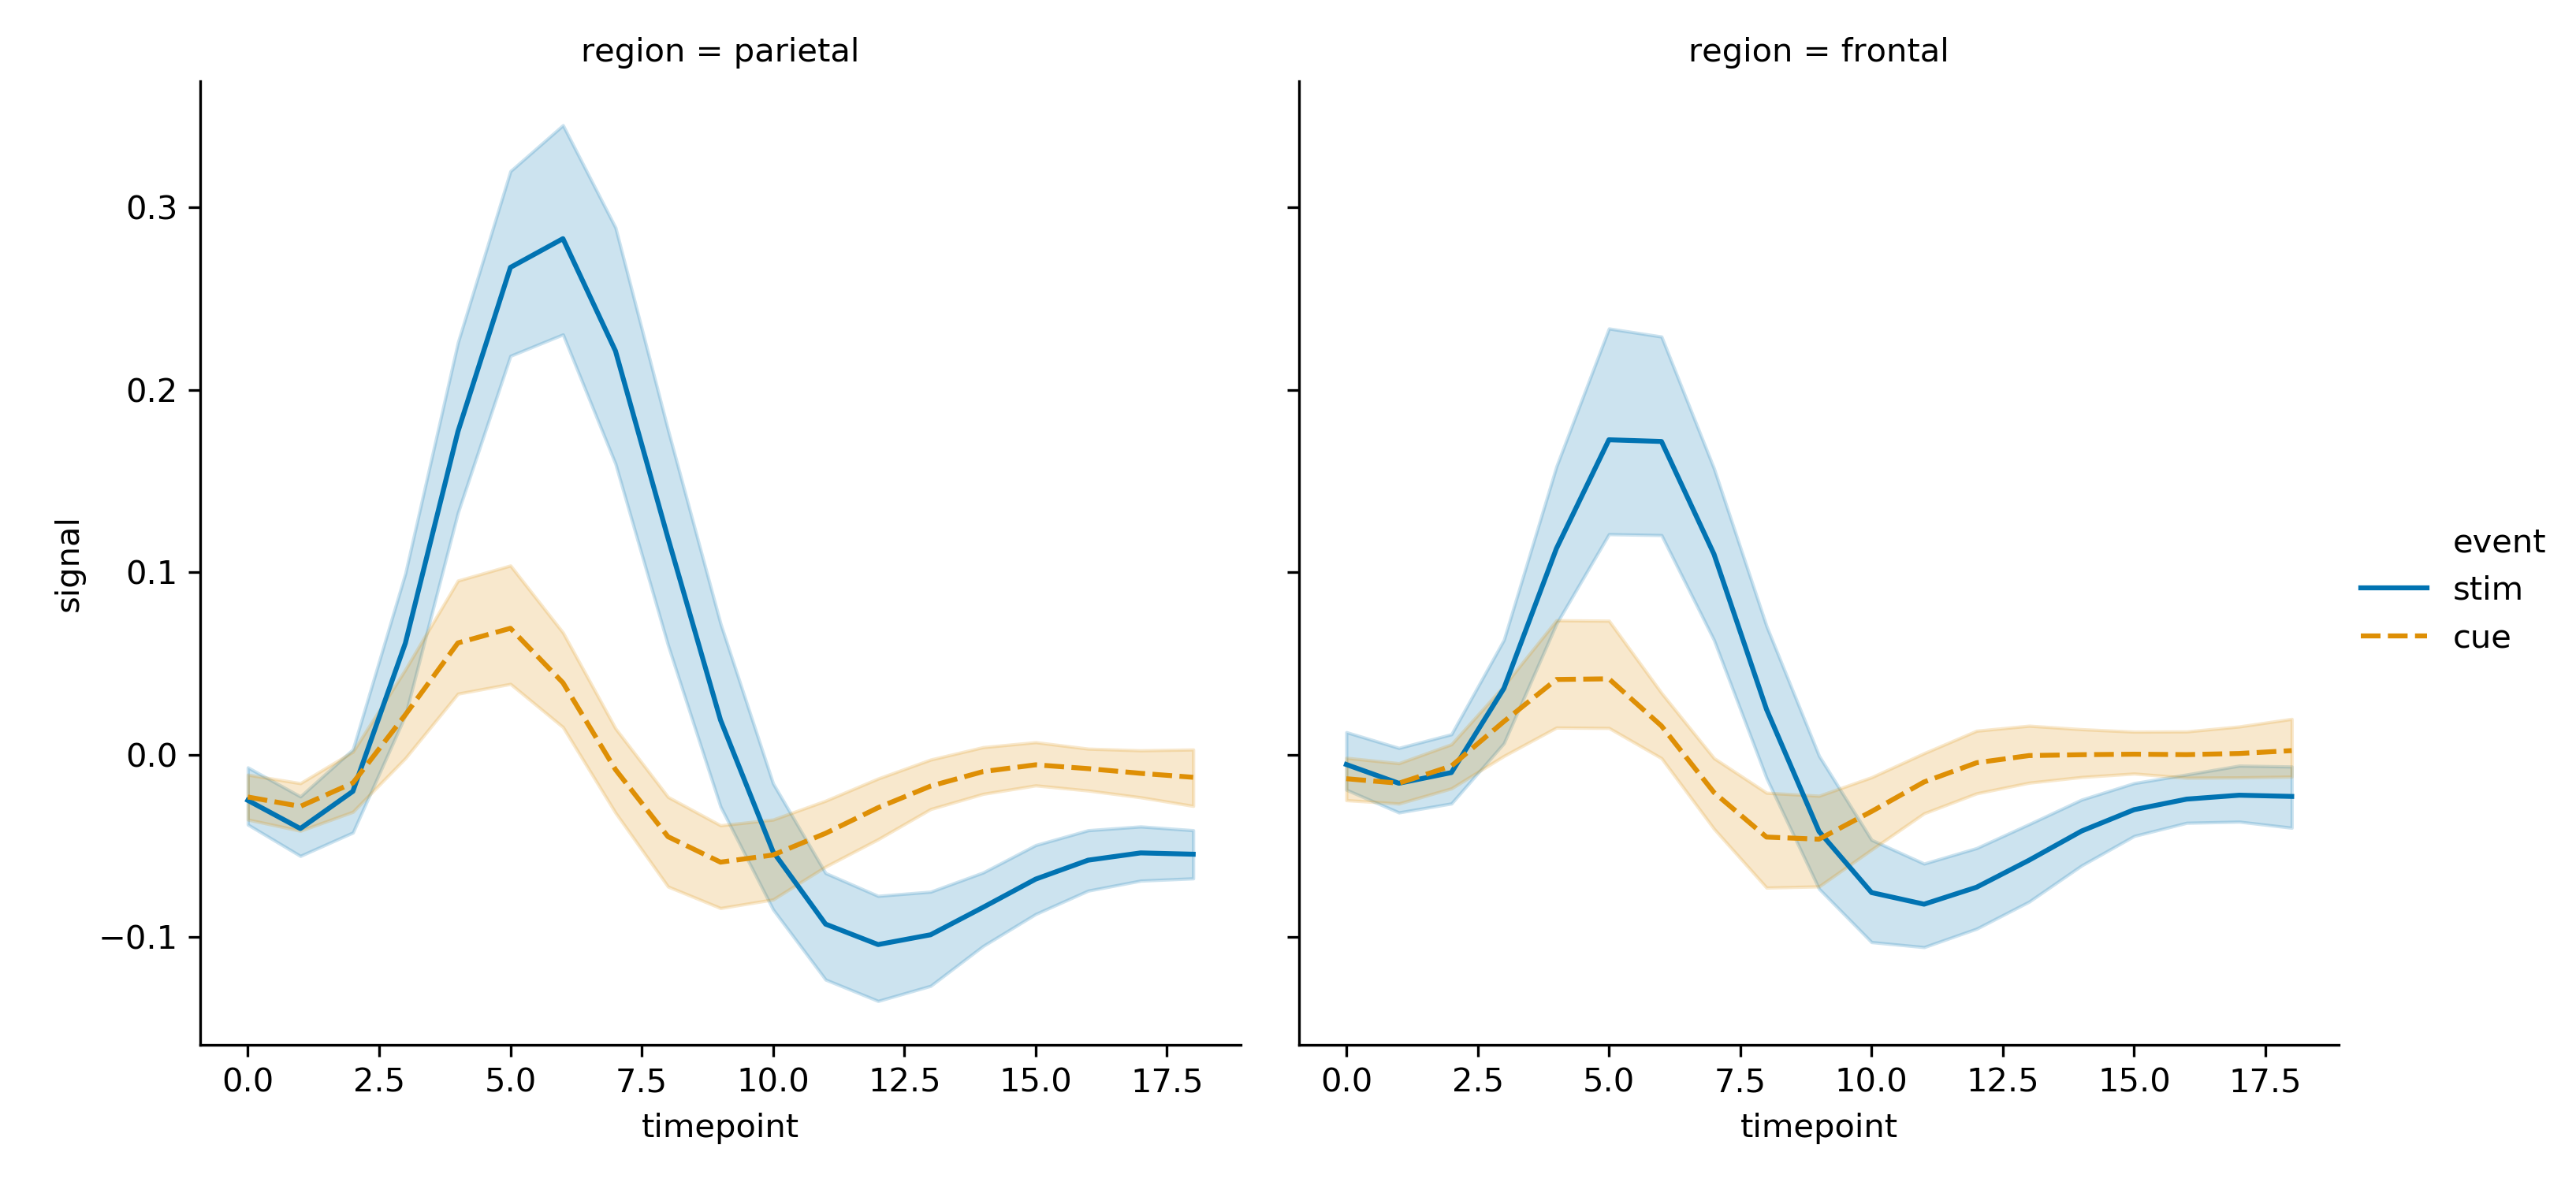
\includegraphics[width = 11cm]{colorblind.png}
        \caption{colorblindness}
        \label{fig:blind}
    \end{figure}
\end{frame}

\subsection{General culture}
\begin{frame}{General culture}
Red stands for tropical zone, yellow stands for temperate zone, blue stands for frigid zone.
    \begin{figure}[htbp]
        \centering
        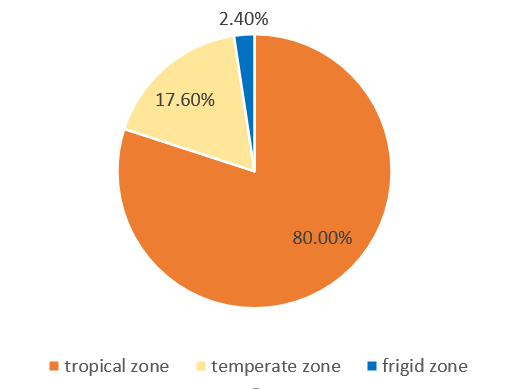
\includegraphics[width = 8cm]{capture.PNG}
        \caption{Biodiversity in different zones on earth}
        \label{fig:my_label}
    \end{figure}  
\end{frame}

\subsection{Warm color and cold color}
\begin{frame}{Warm color and cold color}
Cold color for new cases (bad news) while warm color for vaccinations(good news).
    \begin{figure}
        \centering
        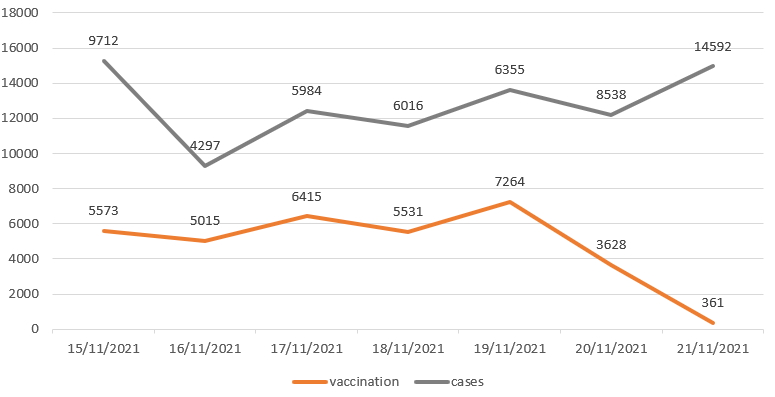
\includegraphics[width = 10cm]{cases.PNG}
        \caption{Covid cases and vaccinations in Switzerland}
        \label{fig:my_label}
    \end{figure}
\end{frame}

\subsection{Specific culture}
\begin{frame}{Specific culture}
China stock market uses red color to reflect prices up and green to reflect prices down.  
    \begin{figure}
        \centering
        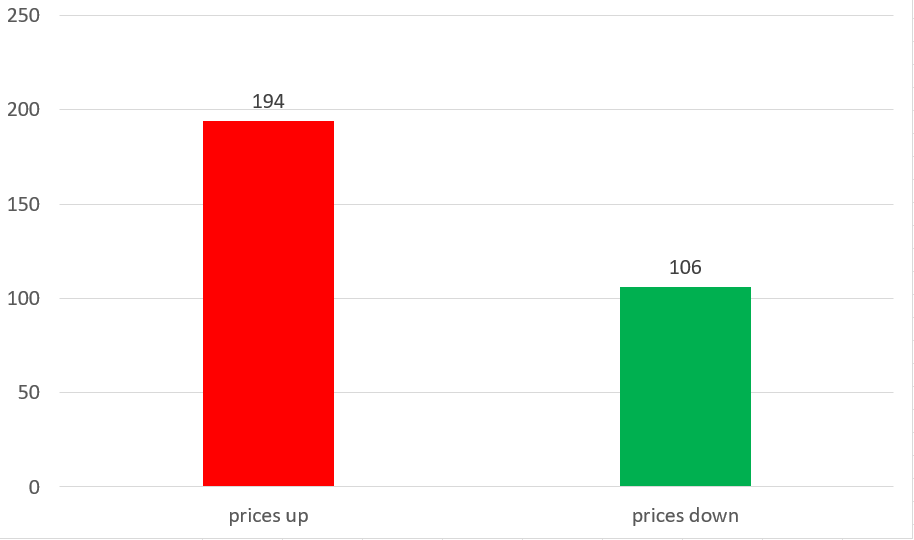
\includegraphics[width = 10cm]{stock.PNG}
        \caption{Prices change of constitute stocks from CSI 300 in 2020}
        \label{fig:my_label}
    \end{figure}
\end{frame}

\subsection{Consistency}
\begin{frame}{Consistency}
    In the above two slides, we added grid to the figures drawn in Excel which forms a pattern in this presentation. Also we added specific numbers in the above three figures(e.g. 194 for prices up and 106 for prices down) which also follows the pattern.
\end{frame}

\section{Tables}
\subsection{Template}
\begin{frame}{Template}
\begin{table}[htbp]
\centering
\begin{tabular}{|c|c|c|c|}
\hline
Table&title1&title2&title3\\ 
\hline
set1&conten1&conten2&conten3\\ 
\hline 
set2&conten1&conten2&conten3\\ 
\hline 
set3&conten1&conten2&conten3\\
\hline
\end{tabular}
\caption{Table Template}
\end{table}
\end{frame}

\subsection{Example of dcolumn}
\begin{frame}{Example of dcolumn}
In order to facilitate observation, we arrange the decimals in the same column of the table by decimal separator alignment. We use LaTeX package dcolumn to implement it.
\begin{table}[htbp]
\centering
\begin{tabular}{c...}
\hline
Weight & \multicolumn{3}{c}{Second-day delivery}                                            \\ \hline
       & \multicolumn{1}{c}{Fedex} & \multicolumn{1}{c}{UPS} & \multicolumn{1}{c}{Airborne} \\
Letter & \$8.00                    & \$6.50                  & \$6.25                       \\
1 lb.  & \$8.00                    & \$7.18                  & \$6.25                       \\
2 lb.  & \$8.79                    & \$8.00                  & \$7.75                       \\
5 lb.  & \$12.14                   & \$10.93                 & \$9.75                       \\
10 lb. & \$18.43                   & \$16.64                 & \$16.00                      \\
50 lb. & \$54.89                   & \$57.11                 & \$58.00                      \\ \hline
\end{tabular}
\caption{List Prices of Express Mail Carriers}
\end{table}
\end{frame}


\section{Equations}
\subsection{Additive Commutative Law}

\begin{frame}
\frametitle{Equations}
\framesubtitle{Additive Commutative Law}
    \begin{equation}
        a+b = b+a
    \end{equation}
for instance:
    \begin{equation}
        \frac{1}{2} + \frac{3}{4} = \frac{3}{4} + \frac{1}{2}
    \end{equation}
\end{frame}

\subsection{Multi-line equations}
\begin{frame}
\frametitle{Equations}
\framesubtitle{Multi-line equations}
    \begin{align*}
        f(x) & = (m+n)^2 \\
             & = m^2+2mn+n^2 \\
    \end{align*}
\end{frame}

\end{document}

